\documentclass[twoside,11pt]{article}

% Any additional packages needed should be included after jmlr2e.
% Note that jmlr2e.sty includes epsfig, amssymb, natbib and graphicx,
% and defines many common macros, such as 'proof' and 'example'.
%
% It also sets the bibliographystyle to plainnat; for more information on
% natbib citation styles, see the natbib documentation, a copy of which
% is archived at http://www.jmlr.org/format/natbib.pdf

\usepackage{jmlr2e}
\usepackage{graphicx}
\graphicspath{{./}}

% Definitions of handy macros can go here

\newcommand{\dataset}{{\cal D}}
\newcommand{\fracpartial}[2]{\frac{\partial #1}{\partial  #2}}
\newcommand{\code}[1]{\texttt{#1}}

% Heading arguments are {volume}{year}{pages}{date submitted}{date published}{paper id}{author-full-names}

% TODO: update heading
\jmlrheading{1}{2000}{1-48}{4/00}{10/00}{meila00a}{Marina Meil\u{a} and Michael I. Jordan}

% Short headings should be running head and authors last names
% TODO: update short heading
\ShortHeadings{TorsionNet}{Jiang, ...}
\firstpageno{1}

\begin{document}

\title{TorsionNet}

% TODO: update authors
\author{\name Runxuan Jiang \email runxuanj@umich.edu \\
       \name Tarun Gogineni \email tgog@umich.edu \\
       \name Josh \\
       \name Ambuj \\
       \name Paul \\
       \addr
       University of Michigan\\
       Ann Arbor, MI 48109, USA} 
% TODO: update editors
\editor{TBD}

\maketitle

\begin{abstract}%   <- trailing '%' for backward compatibility of .sty file
  We propose \code{TorsionNet}, an open-source deep reinforcement learning library designed for molecular conformer generation using Python. \code{TorsionNet} features several pre-built environments and baseline agents based on state-of-the-art algorithms in the field. The environments and agents are built on a modular interface, allowing users to easily build and test new implementations. Additionally, \code{TorsionNet} comes with extensive logging and visualization tools for evaluation of agents and generated conformers, as well as a toolkit for generating and modifying molecules. \code{TorsionNet} is well-tested and thoroughly documented, and is available through on PyPi and on Github: \code{https://github.com/ZimmermanGroup/conformer-ml}.
\end{abstract}

\begin{keywords}
  reinforcement learning, deep learning, deep reinforcement learning, open source, conformer generation, computational chemistry
\end{keywords}

\section{Introduction}
There have been many recent developments in the use of deep reinforcement learning applied to computational chemistry tasks \citep{li2018foldingzero,zhou2017reactions,simm2020moldesign}. One such task is conformer generation \citep{gogineni2020torsionnet}, which involves finding an ensemble of unique low-energy three-dimensional orientations, or conformers, for a given molecule \citep{ebejer2020confgen}. Efficient and accurate prediction of low-energy conformers is integral to molecular modeling, with wide applications from drug development to 3D QSAR \citep{cole2018confgen}. However, there currently exists very few open-source software libraries for deep learning applied conformer generation, and the ones that do exist are often not modular enough for further experimentation and modification. Thus, we introduce \code{TorsionNet}, a comprehensive and modular Python library for applying deep reinforcement learning to conformer generation, using PyTorch \citep{torch} for deep learning and RDKit for chemoinformatic capabilities.

Many libraries already exist that contain benchmarking experiments and baseline implementations for general deep reinforcement learning. For example, OpenAI Gym \citep{brockman2016gym} and bsuite \citep{osband2020bsuite} both contain implementations of reinforcement learning environments commonly used for benchmarking agents, such as cartpole, mountaincar, and Atari. \code{TorsionNet} seeks to fill this role within the conformer generation space by supplying pre-built environments for benchmarking agents, as well as an interface to easily customize environments for further exploration. This allows \code{TorsionNet}'s environment to be readily modified for other chemoinformatic tasks related to conformer generation, such as protein folding and reaction prediction.

There are also many implementations of baseline deep reinforcement learning agents available, such as Rllib \citep{liang2018rllib} and OpenAI baselines \citep{dhariwal2018baselines}. However, due to the complex nature of molecules which are often represented by graph structures rather than vectors, a large amount of modification and setup work is required to adapt these baseline libraries to work with molecule environments. Within \code{TorsionNet}, several baseline training algorithms are implemented to accomodate generalized observation spaces, as well as baseline neural networks for molecule inputs built with graph neural network (GNN) components using PyTorch Geometric \citep{fey2019geometric}.

Additionally, \code{TorsionNet} provides extensive logging capabilities and an analysis module for recording and visualizing training results, including conformer-generation specific metrics and visuals.

\section{TorsionNet Architecture}

  \begin{figure}[h]
    \centering
    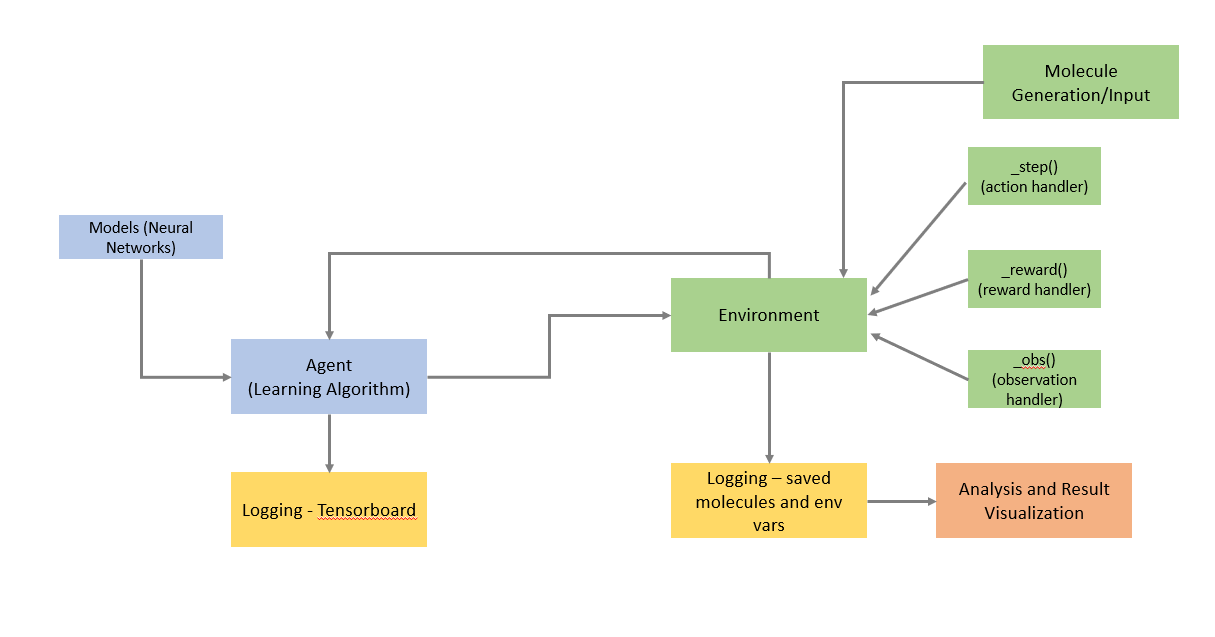
\includegraphics[width=\textwidth]{architecture.png}
    \caption{Architecture of \code{TorsionNet}. Agent components are colored blue, environment components are colored green, and logging/analysis componenets are colored yellow.}
  \end{figure}

\subsection{Environments}
All \code{TorsionNet} environments are classes built by overriding methods of the \code{ConformerEnv} base class. The main methods to be overridden are the \code{\_step(action)} method, which specifies how the environment will modify its state/molecule given an action input, the \code{\_obs()} method, which converts the environment's state into an input for a neural network, and the \code{\_reward()} method, which calculates the reward from the current state of the environment. Other functions such as \code{\_done()}, which determines the end of an episode in the environment, and \code{reset()} can also be overridden at the user's convenience.

To demonstrate the flexibility of the \code{ConforomerEnv} interface, \code{TorsionNet} implements several different mixin classes overriding one of the previously mentioned methods, which can then be mixed and matched to form new environments, some of which are included as pre-built environments in \code{TorsionNet}, including the environment used in \citet{gogineni2020torsionnet}.

  \subsubsection{Molecule Generation}
  All \code{TorsionNet} environments are initialized with a \code{MolConfig} object, which specifies the molecule to be used in the environment as well as any molecule-specific parameters needed by the environment. This allows environments to be compatible with any molecule, including user-generated molecules.

  Additionally, \code{TorsionNet} contains scripts for generating \code{MolConfig} objects for several simple molecules and molecule benchmarks found in \citet{gogineni2020torsionnet}, such as branched alkanes, lignin, and more.

\code{TorsionNet} also includes wrappers for executing multiple environments in parallel. 

\subsection{Agents}
  \code{TorsionNet} contains implementations of several baseline agents, as well as an interface for creating custom agents \code{BaseAgent}. Agents implement the \code{step()} method of \code{BaseAgent}, which correspond to one iteration of interacting with the environment to collect samples and then training on those samples.

  Agents are initialized with a \code{Config} object, which specifies the neural network to be used, as well as training hyperparameters. Agents can also be configured with an evaluation environment, in which the agent will not interact with while training but will be evaluated on the evaluation environment every certain number of steps.

  \code{TorsionNet} implements several baseline built-in agents, including recurrent and non-recurrent implementations of advantage actor critic (A2C) \citep{wu2017a2c} and proximal policy optimization (PPO) \citep{schulman2017ppo}.

  \subsubsection{Models}
    \code{TorsionNet} implements several baseline built-in neural network models, including recurrent and non-recurrent versions of the \code{TorsionNet} model from \citep{gogineni2020torsionnet} which utilizes a message passing neural network (MPNN) \citep{gilmer2017mpnn}, as well as similar graph networks that utilize graph attention networks \citep{gatnn}.


\subsection{Logging and Analysis}

\section{Future Work}
pass
\section{Conclusions}
pass



% Acknowledgements should go at the end, before appendices and references

\acks{We would like to acknowledge ...}

\vskip 0.2in
\bibliography{reference}


% Manual newpage inserted to improve layout of sample file - not
% needed in general before appendices/bibliography.

\newpage

\appendix
\section*{Appendix A.}

\end{document}